\documentclass[border=12pt]{standalone}
\usepackage{pgfplots}
\pgfplotsset{compat=1.18, trig format plots=deg}
\definecolor{ccyl}{HTML}{2E6DA4}
\definecolor{cpla}{HTML}{D98E20}
\definecolor{cxz}{HTML}{3E8E4E}
\begin{document}
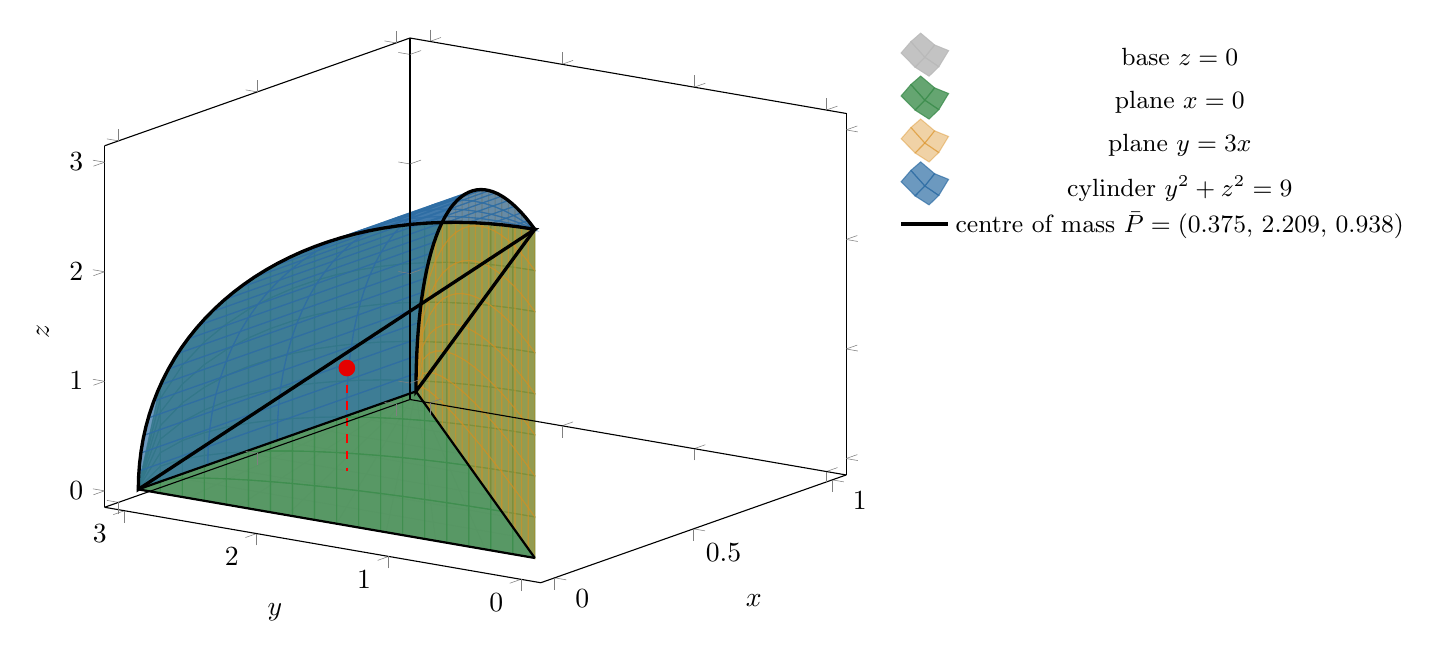
\begin{tikzpicture}
\begin{axis}[
    view={-55}{20}, width=11cm, height=8.5cm,
    axis on top, grid=none, tick align=outside,
    xlabel=$x$, ylabel=$y$, zlabel=$z$,
    xmin=0,xmax=1, ymin=0,ymax=3, zmin=0,zmax=3,
    xtick={0,0.5,1}, ytick={0,1,2,3}, ztick={0,1,2,3},
    enlargelimits=0.05, clip=false,
    every axis plot post/.append style={shader=flat},
    legend style={at={(axis description cs:1.06,1.02)}, anchor=north west,
                  draw=none, font=\small, align=left, fill=none},
    legend image post/.append style={draw=black, thick}]
    % base z=0
    \addplot3[surf, gray!55, opacity=0.85, domain=0:1, y domain=0:1, samples=9, samples y=9]
        ({x},{3*x+(1-x)*3*y},{0});
    \addlegendentry{base $z=0$};
    % plane x=0
    \addplot3[surf, cxz, opacity=0.80, domain=0:1, y domain=0:1, samples=19, samples y=9]
        ({0},{3*x},{3*sqrt(1-x^2)*y});
    \addlegendentry{plane $x=0$};
    % plane y=3x
    \addplot3[surf, cpla, opacity=0.40, domain=0:1, y domain=0:1, samples=19, samples y=9]
        ({x},{3*x},{3*sqrt(1-x^2)*y});
    \addlegendentry{plane $y=3x$};
    % cylinder wall
    \addplot3[surf, ccyl, opacity=0.70, domain=0:90, y domain=0:1, samples=29, samples y=5]
        ({sin(x)*y},{3*sin(x)},{3*cos(x)});
    \addlegendentry{cylinder $y^2+z^2=9$};
    % edges
    \addplot3[very thick, black, domain=0:90, samples=41, variable=t] ({sin(t)},{3*sin(t)},{3*cos(t)});
    \addplot3[very thick, black, domain=0:90, samples=41, variable=t] ({0},{3*sin(t)},{3*cos(t)});
    \addplot3[thick, black] coordinates {(0,0,0) (0,3,0)};
    \addplot3[thick, black] coordinates {(0,0,0) (1,3,0)};
    \addplot3[thick, black] coordinates {(0,3,0) (1,3,0)};
    % centre of mass
    \addplot3[red, dashed, thick] coordinates {(0.3747,2.2089,0.9375) (0.3747,2.2089,0)};
    \addplot3[only marks, mark=*, mark size=2.8, red!90!black] coordinates {(0.3747,2.2089,0.9375)};
    \addlegendentry{centre of mass $\bar P=(0.375,\,2.209,\,0.938)$};
\end{axis}
\end{tikzpicture}
\end{document}
